\begin{figure}
	\centering
	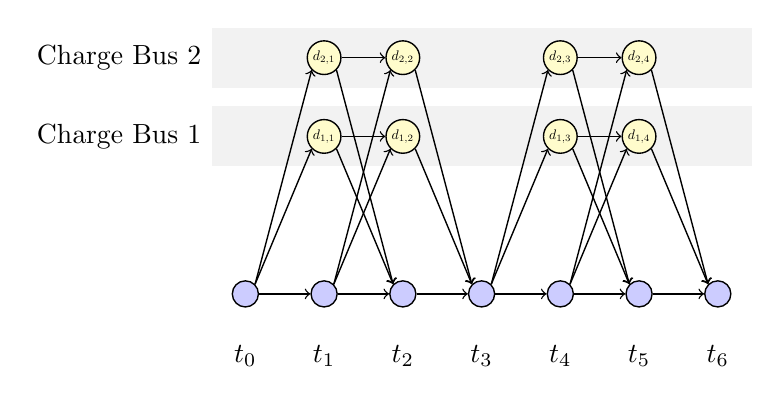
\begin{tikzpicture} 

		\node[rectangle, fill=gray!10, minimum width=2.7in, minimum height=.3in,label=left:Charge Bus 2](bus2Box) at (3,3){};
		\node[rectangle, fill=gray!10, minimum width=2.7in, minimum height=.3in,label=left:Charge Bus 1](bus1Box) at (3,2){};

		\node[circle, fill=blue!20, line width=0.5pt, draw=black, minimum size=0.1in](one) at (0,0){};
		\node[circle, fill=blue!20, line width=0.5pt, draw=black, minimum size=0.1in](two) at (1,0){}; 
		\node[circle, fill=blue!20, line width=0.5pt, draw=black, minimum size=0.1in](three) at (2,0){};
		\node[circle, fill=blue!20, line width=0.5pt, draw=black, minimum size=0.1in](four) at (3,0){};
		\node[circle, fill=blue!20, line width=0.5pt, draw=black, minimum size=0.1in](five) at (4,0){};
		\node[circle, fill=blue!20, line width=0.5pt, draw=black, minimum size=0.1in](six) at (5,0){};
		\node[circle, fill=blue!20, line width=0.5pt, draw=black, minimum size=0.1in](seven) at (6,0){};
		
		\node[circle, fill=yellow!20, line width=0.5pt, draw=black, minimum size=0.1in, inner sep=1pt](eight) at (1,2){\scalebox{0.5}{$d_{1,1}$}};
		\node[circle, fill=yellow!20, line width=0.5pt, draw=black, minimum size=0.1in, inner sep=1pt](nine) at (2,2){\scalebox{0.5}{$d_{1,2}$}};
		\node[circle, fill=yellow!20, line width=0.5pt, draw=black, minimum size=0.1in, inner sep=1pt](ten) at (4,2){\scalebox{0.5}{$d_{1,3}$}}; 
		\node[circle, fill=yellow!20, line width=0.5pt, draw=black, minimum size=0.1in, inner sep=1pt](eleven) at (5,2){\scalebox{0.5}{$d_{1,4}$}}; 

		\node[circle, fill=yellow!20, line width=0.5pt, draw=black, minimum size=0.1in, inner sep=1pt](twelve) at (1,3){\scalebox{0.5}{$d_{2,1}$}};
		\node[circle, fill=yellow!20, line width=0.5pt, draw=black, minimum size=0.1in, inner sep=1pt](thirteen) at (2,3){\scalebox{0.5}{$d_{2,2}$}};
		\node[circle, fill=yellow!20, line width=0.5pt, draw=black, minimum size=0.1in, inner sep=1pt](fourteen) at (4,3){\scalebox{0.5}{$d_{2,3}$}}; 
		\node[circle, fill=yellow!20, line width=0.5pt, draw=black, minimum size=0.1in, inner sep=1pt](fifteen) at (5,3){\scalebox{0.5}{$d_{2,4}$}}; 

		\draw [->, line width=0.5pt] (one.east) -- (two.west);
		\draw [->, line width=0.5pt] (two.east) -- (three.west);
		\draw [->, line width=0.5pt] (three.east) -- (four.west);
		\draw [->, line width=0.5pt] (four.east) -- (five.west);
		\draw [->, line width=0.5pt] (five.east) -- (six.west);
		\draw [->, line width=0.5pt] (six.east) -- (seven.west);

		\draw [->, line width=0.5pt] (one.north east) -- (eight.south west);
		\draw [->, line width=0.5pt] (two.north east) -- (nine.south west);
		\draw [->, line width=0.5pt] (four.north east) -- (ten.south west);
		\draw [->, line width=0.5pt] (five.north east) -- (eleven.south west);
		\draw [->, line width=0.5pt] (eight.south east) -- (three.north west);
		\draw [->, line width=0.5pt] (nine.south east) -- (four.north west);
		\draw [->, line width=0.5pt] (ten.south east) -- (six.north west);
		\draw [->, line width=0.5pt] (eleven.south east) -- (seven.north west);
		\draw [->, line width=0.5pt] (eight.east) -- (nine.west);
		\draw [->, line width=0.5pt] (ten.east) -- (eleven.west); 

		\draw [->, line width=0.5pt] (one.north east) -- (twelve.south west);
		\draw [->, line width=0.5pt] (two.north east) -- (thirteen.south west);
		\draw [->, line width=0.5pt] (four.north east) -- (fourteen.south west);
		\draw [->, line width=0.5pt] (five.north east) -- (fifteen.south west);
		\draw [->, line width=0.5pt] (twelve.south east) -- (three.north west);
		\draw [->, line width=0.5pt] (thirteen.south east) -- (four.north west);
		\draw [->, line width=0.5pt] (fourteen.south east) -- (six.north west);
		\draw [->, line width=0.5pt] (fifteen.south east) -- (seven.north west);
		\draw [->, line width=0.5pt] (twelve.east) -- (thirteen.west);
		\draw [->, line width=0.5pt] (fourteen.east) -- (fifteen.west); 

		\node[rectangle, minimum width=0.3in, minimum height=1.2in,label=below:$t_0$](time0Box) at (0,1){};
		\node[rectangle, minimum width=0.3in, minimum height=1.2in,label=below:$t_1$](time1Box) at (1,1){};
		\node[rectangle, minimum width=0.3in, minimum height=1.2in,label=below:$t_2$](time2Box) at (2,1){};
		\node[rectangle, minimum width=0.3in, minimum height=1.2in,label=below:$t_3$](time3Box) at (3,1){};
		\node[rectangle, minimum width=0.3in, minimum height=1.2in,label=below:$t_4$](time4Box) at (4,1){};
		\node[rectangle, minimum width=0.3in, minimum height=1.2in,label=below:$t_5$](time5Box) at (5,1){};
		\node[rectangle, minimum width=0.3in, minimum height=1.2in,label=below:$t_6$](time6Box) at (6,1){}; 
	\end{tikzpicture}
	\caption{SOC indicators}
	\label{fig:socDiagram}
\end{figure}

